% Conditional expectation as an orthogonal projection onto L^2(G). Generated by a short script.
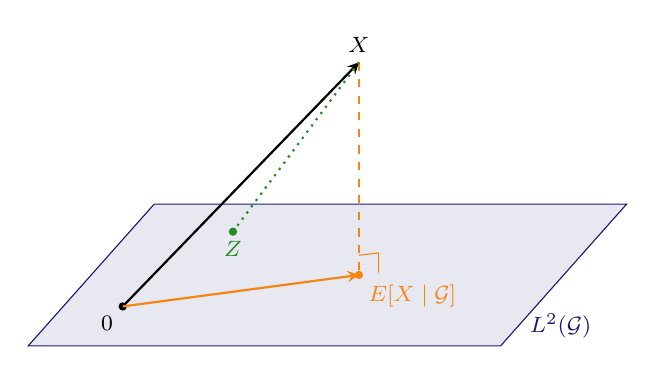
\begin{tikzpicture}[>=stealth,every node/.style={font=\footnotesize}]
\fill[MidnightBlue!10] (0,0)--(6,0)--(7.6,1.8)--(1.6,1.8)--cycle;
\draw[MidnightBlue] (0,0)--(6,0)--(7.6,1.8)--(1.6,1.8)--cycle;
\node[MidnightBlue,anchor=west] at (6.25,0.25) {$L^2(\mathcal G)$};
\coordinate (O) at (1.2,0.5);
\coordinate (Y) at (4.2,0.9);
\coordinate (X) at (4.2,3.6);
\coordinate (Z) at (2.6,1.45);
\fill (O) circle (1.5pt) node[below left] {$0$};
\draw[->,thick] (O)--(X) node[above] {$X$};
\draw[->,thick,BurntOrange] (O)--(Y);
\fill[BurntOrange] (Y) circle (1.5pt) node[below right] {$\mathbb E[X\mid\mathcal G]$};
\draw[dashed,thick,BurntOrange] (X)--(Y);
\draw[BurntOrange] (4.2,1.15)--(4.45,1.18)--(4.45,0.93);
\fill[ForestGreen] (Z) circle (1.5pt) node[below] {$Z$};
\draw[dotted,thick,ForestGreen] (X)--(Z);
\end{tikzpicture}
